\chapter{Design}
\label{chap:design}

This chapter introduces \emph{\memsc}, an alternative method for invoking
\llinux system calls. The main design points are presented along with the
overall architecture of the system. Additionally, the way \memsc can be used is
explained and some example code snippets are given.

\section{Overview}

The current system call forwarding mechanism using inter-processor interrupts,
described in Section \ref{sec:syscall_forwarding}, is a significant performance
bottleneck for applications issuing large amounts of system calls. For this
purpose, \emph{\memsc} has been developed as an alternative way to forward
system calls from decoupled \llinux threads using shared memory.

The general idea is that decoupled threads can post system calls in special
memory pages while \llinux is constantly polling memory in order to detect
changes in those pages. Once \llinux encounters new system calls, it
immediately executes them on behalf of the appropriate thread. When execution
is complete, the result is written back to memory for the requesting thread to
pick it up from there.

Even though the main goal is faster system call forwarding in general, \memsc
can provide applications willing to directly use its API with further benefits
such as system call batching and asynchronous system calls. This works by
allowing applications to post multiple system calls in memory at once before
blocking and waiting for their processing.

In general, system calls need not happen in a synchronous matter. Applications
don't necessarily have to block when issuing a system call. Instead, a new
entry can be simply written to memory while the application proceeds with other
useful user-space work. At a later point in time, the application can check if
a system call it has previously issued is complete in order to pick up its
return value.

Using \memsc for system processes is optional. That means that some programs
can opt to use \memsc, while others can still forward their system calls using
the traditional way that uses L4 IPC. It is even possible to combine the two
mechanisms and have some system calls be forwarded using one of them and some
using the other. Detached threads that want to register for \memsc services
simply need to invoke the new \emph{memsc\_register()} system call which was
added to \llinux as part of \memsc. It is worth noting that even non-decoupled
processes can use \memsc, however this only makes sense when they want to use
its asynchronous system call execution model.

\section{The Syspage}

Every user process using \memsc posts its system calls in a special memory page
called the \emph{\sysp}. The \sysp is nothing more than a regular memory page
that is shared between the user-space and the kernel-space in order to be
readable and writeable from both \llinux and the corresponding detached user
thread. Each user process registered for \memsc services has its own \sysp.

\begin{figure}[h]
\centering
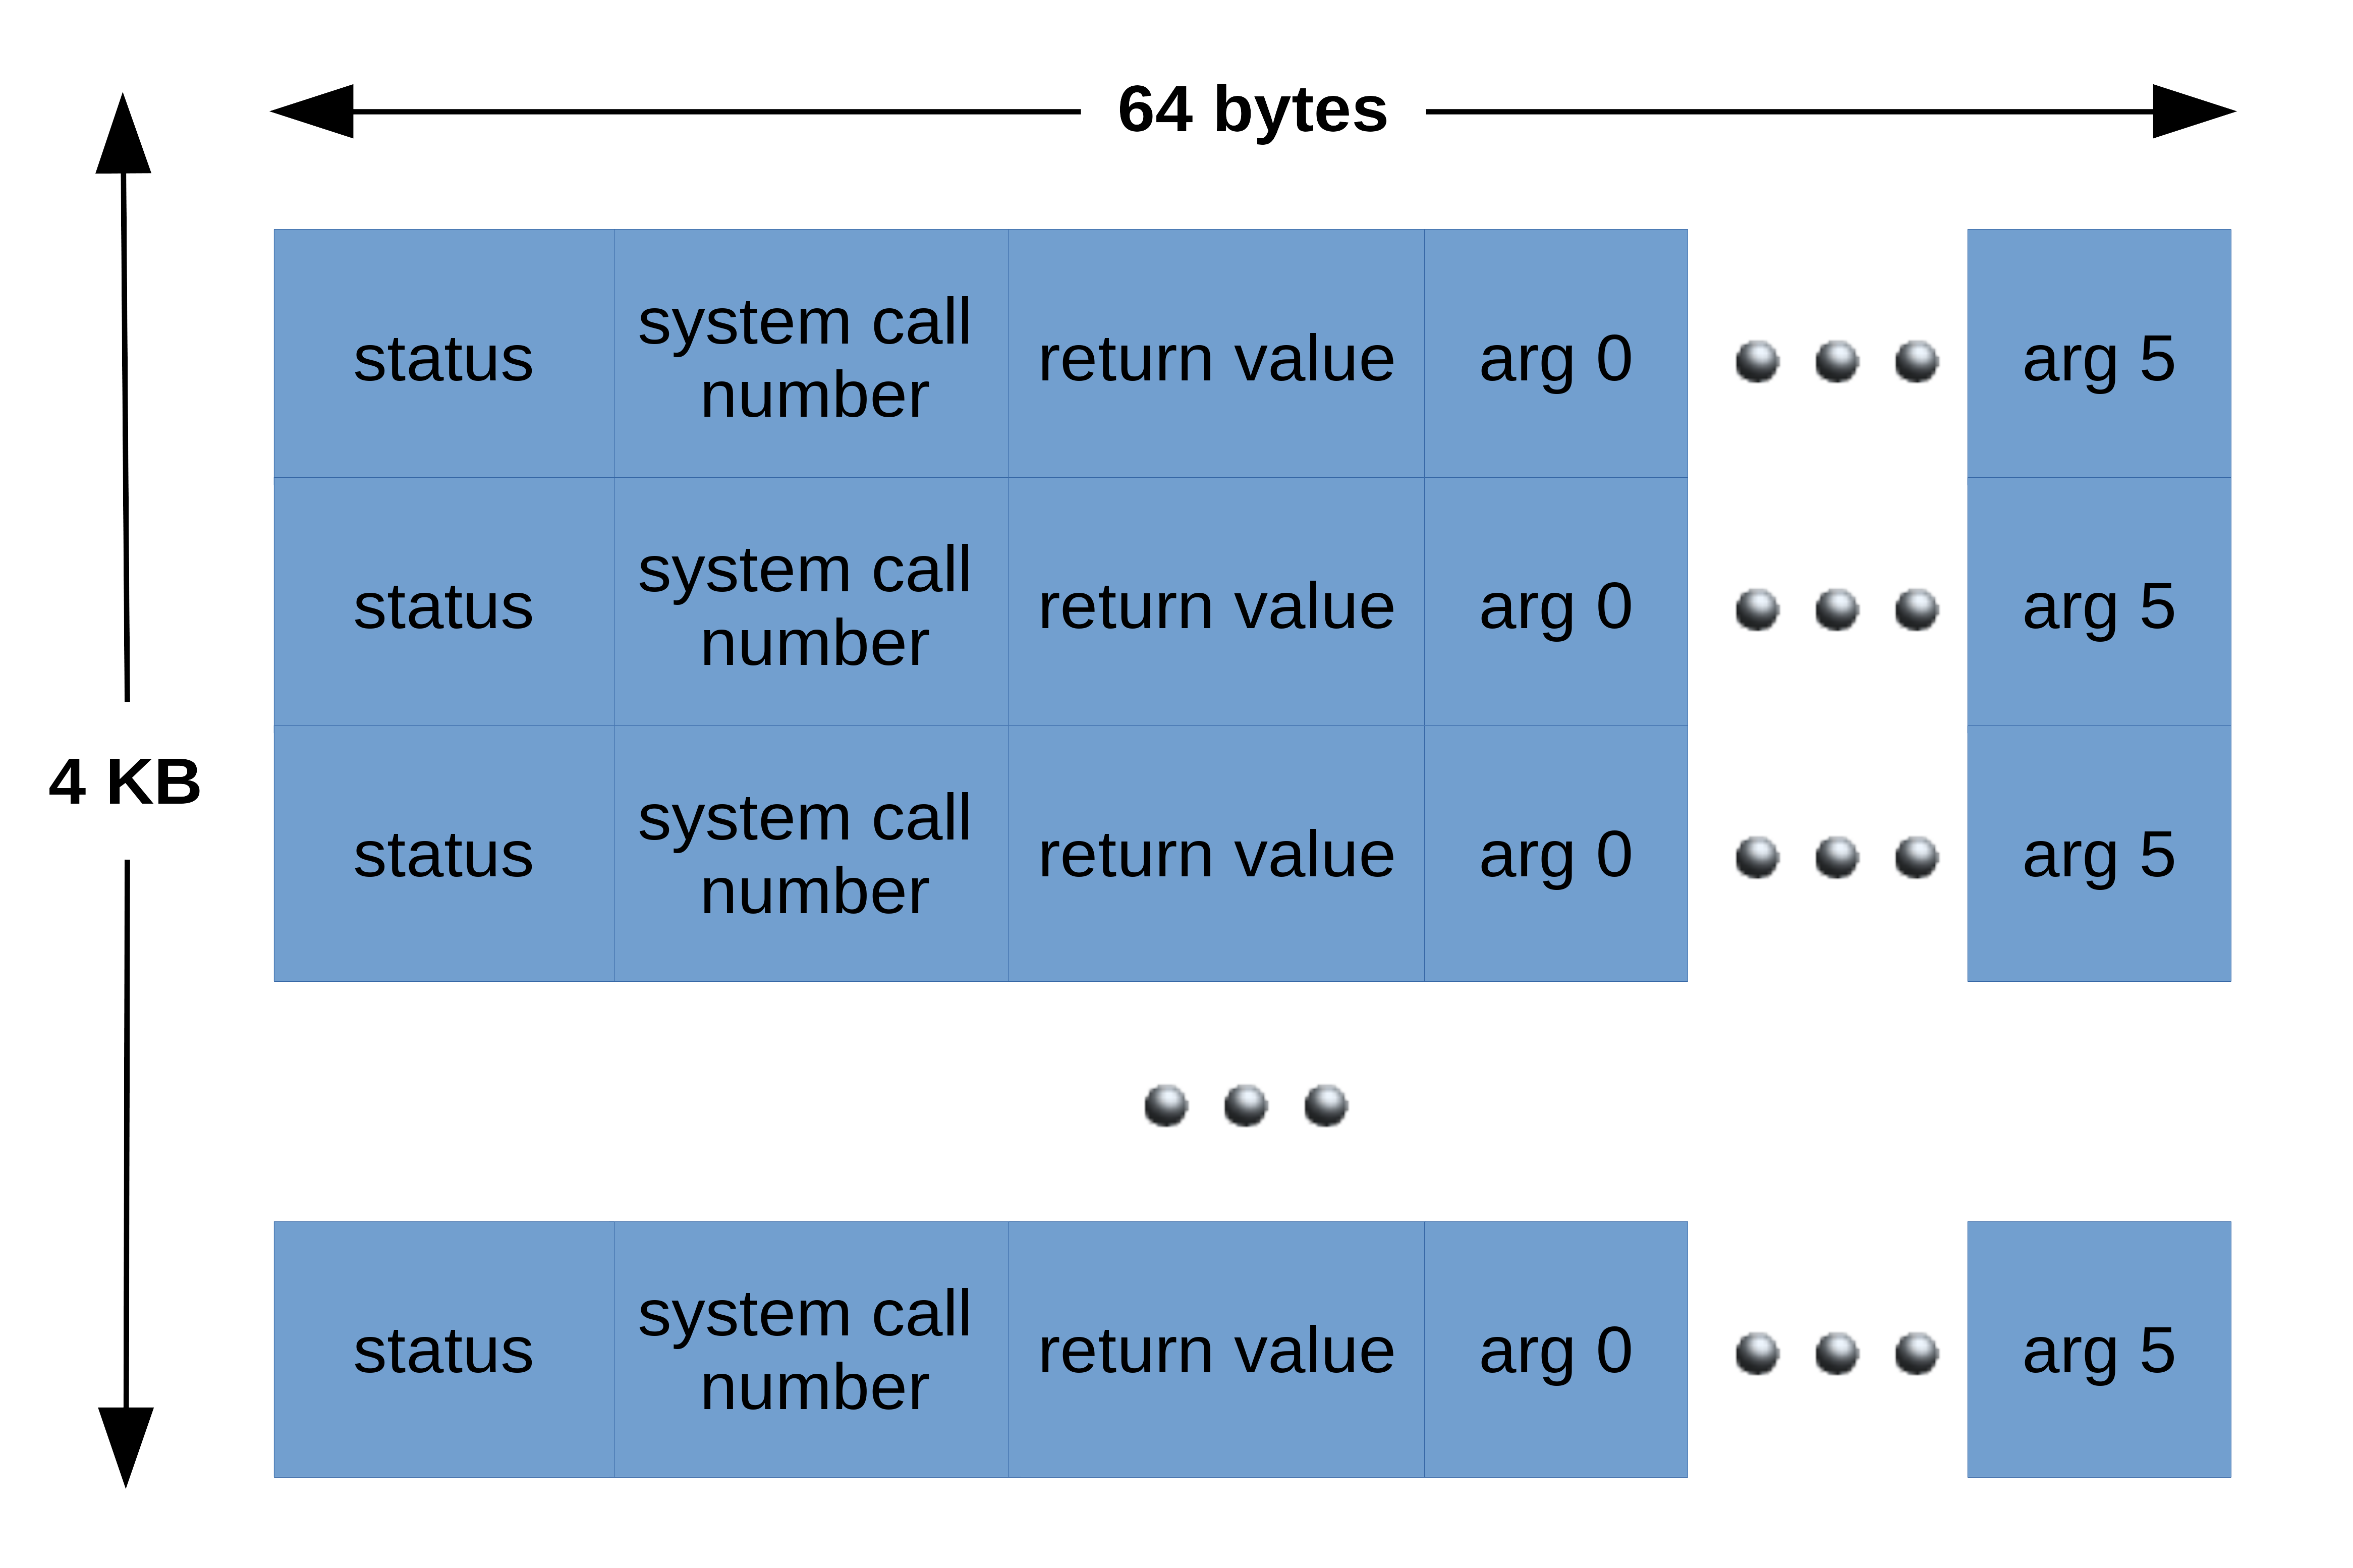
\includegraphics[scale=0.075]{syspage}
\caption{A syspage consisting of multiple system call entries}
\label{fig:syspage}
\end{figure}

The \sysp can be viewed as a table of adjacent system call entries. Each entry
consists of an entry status, the system call number, the system call arguments
(which can be up to 6 according to the Linux ABI), and the return value for
when the system call has been processed by the kernel.

Entries of this table can be a) \emph{free} meaning that that slot of the table
is available for posting a new system call, b) \emph{submitted} meaning that
the user-space has already posted a system call but its result is not yet
available, and c) \emph{done} meaning that the system call has been processed
and its result is available. This is determined by the status field of each
entry.

Figure \ref{fig:syspage} illustrates a syspage in a system with a memory page
size of 4KB which is the most common page size. Syspage entries have been
designed to occupy exactly 64 bytes in order to match the cache line width of
modern CPUs and avoid false sharing. As a result, in such a system, a maximum
of 64 unprocessed system call entries could be posted before running out of
slots in the \sysp.

The \sysp is implemented as a circular buffer also known as ring buffer. That
means that entries are processed by the kernel in the same order they have been
submitted. Hence, if a user thread posts multiple entries and later finds that
one of them has been processed, it automatically knows that all entries posted
before that one have been processed as well.

\section{The Scanner Thread}

As mentioned in the previous sections, \llinux needs to be constantly polling
memory in order to detect newly posted system calls. This exactly is the job of
the \emph{scanner} thread, an \llinux kernel thread dedicated to this task.

The scanner is constantly checking all the registered \sysp{s} for updates in a
round-robin fashion. Since as mentioned in the previous section a \sysp is
actually a ring buffer, only the head entry of that buffer needs to be checked
on each iteration. Hence, the scanner does not need to perform a full scan of
each \sysp every time.  It simply needs to ``scan'' all registered \sysp{s} by
checking their head entry only.

No other task is performed by the scanner, nor does it execute system calls
that it finds in the scanning process. Instead, once the scanner actually
encounters an unprocessed entry, it simply dispatches the work to some other
thread in the system and continues by scanning the rest of the pages.

The scanner thread does not need to run at all times. It is automatically
spawned when needed (ie when \memsc services are initially requested) and it is
terminated once there are no more \memsc processes in order to not consume
system resources. A single scanner thread is sufficient for a large number of
registered processes, since as explained above the scanning process is fast.

\section{Worker Threads}
\label{section:workers}

Memsc worker threads are \llinux kernel threads that execute system calls on
behalf of user processes. Each worker thread is associated with a single user
process and each user process has a unique worker thread executing its system
calls. Worker threads are able to execute system calls for a certain process by
accessing the same address space as that process.

These threads sleep for as long as there is no work for them to process.
However, once the scanner thread detects a new system call on a syspage, it
immediately wakes up the corresponding memsc worker thread in order to be
scheduled as soon as possible.

Once a worker thread wakes up, it executes all pending system calls found in
its ring buffer, not just the first one. This way, worker threads enable batch
processing of system calls. When a worker finishes all the work that it finds
on its \sysp it goes back to sleep, waiting for the scanner thread to wake it
up again once more work is available.

\section{Architecture}

A visual representation of the system architecture with \memsc is depicted in
Figure \ref{fig:architecture}. A system with 4 physical CPUs and 2 vCPUs
sitting on the last 2 physical cores is used in this example. A decoupled
thread that has registered for \memsc services runs on CPU 0, outside of
\llinux's scope. Its \memsc worker thread along with its corresponding
kernel-side context described in section \ref{sec:decoupling} are managed by
\llinux and their execution is multiplexed in vCPU1. All 3 threads can access
the same memory and they run in the same context from the perspective of
\llinux.

\begin{figure}[h]
\centering
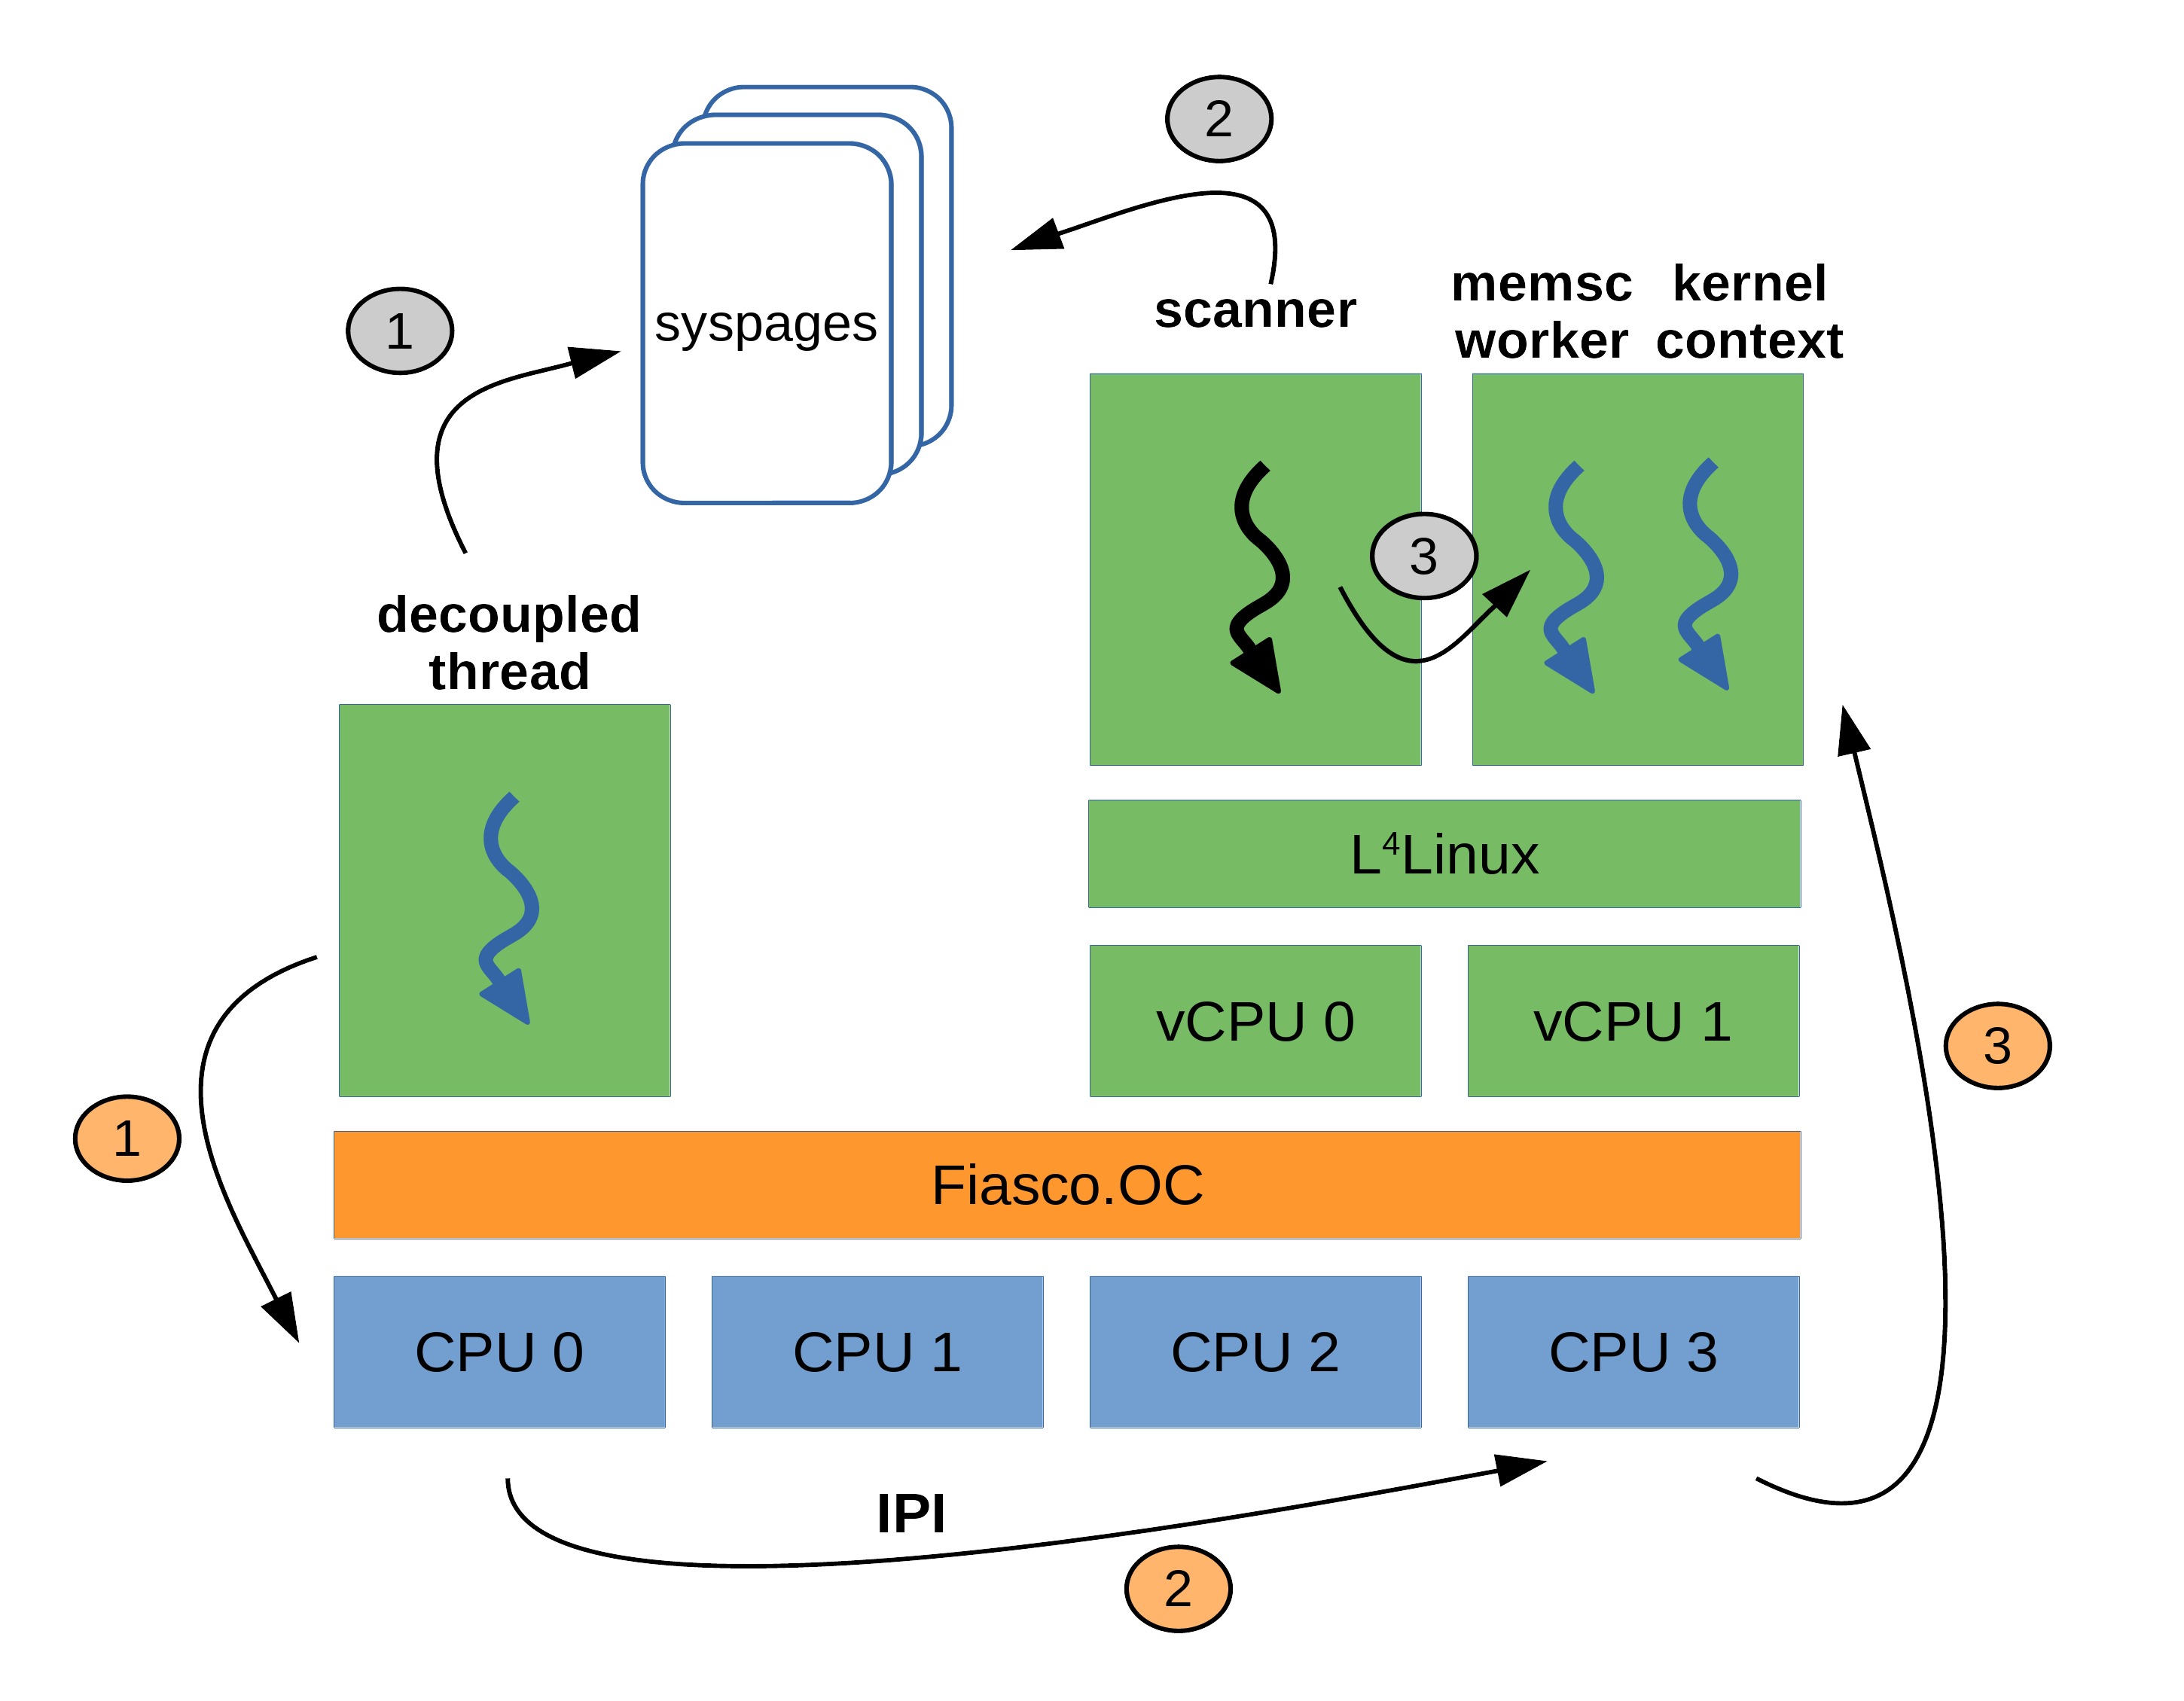
\includegraphics[scale=0.15]{architecture}
  \caption{Memsc in action. System calls are forwarded via syspages (gray)
  while other exceptions are forwarded in the traditional way using L4 IPC
  (orange). Threads in blue run in the same context from the perspective of
  \llinux. }
\label{fig:architecture}
\end{figure}

The decoupled thread might need to enter the \llinux kernel in the following
cases; when it invokes system calls, when a hardware interrupt is received (for
example the network card notifies that a new network packet has arrived) and
when a software exception is raised (for example due to a page fault).
Traditionally, all these kinds of events would be forwarded to \llinux in the
way described in section \ref{sec:syscall_forwarding}. The software or hardware
exception traps into Fiasco in CPU 0, which notifies the Fiasco instance
running on CPU 3 using an inter-processor interrupt. Fiasco on that core then
forwards it to vCPU1 and finally \llinux wakes up the appropriate kernel-side
context to handle the exception.

The process for invoking system calls using \memsc is different. The decoupled
thread first posts one or more system call entries on its syspage. The scanner
thread running on its dedicated vCPU constantly scans all syspages. Once it
detects a change, it immediately wakes up the corresponding worker thread in
order to execute the system call. Note that neither the L4Re microkernel nor
the kernel-side context are involved now in system call invocations.  However,
all kinds of exceptions\footnote{ system calls are now exception-less} are
still forwarded using the traditional way.

Using this architecture requires an additional kernel thread for each decoupled
\llinux process. Nonetheless, this does not really add any noteworthy overhead.
The memory footprint of the extra thread is negligible anyway and Linux's
Completely Fair Scheduler (CFS) requires constant time for choosing a thread
for execution independently of the total amount of threads present in the
system.

\subsection{Parallel Execution of User and Kernel Code}

An interesting aspect of this architecture is that it allows user-space code
and kernel-space code execution of the same process in parallel. The decoupled
thread, can post a few system call entries on its \sysp and continue executing
user-space code. At the same time, having being woken up by the scanner, the
\memsc worker can execute system calls for the same process in parallel.

This eliminates any blocked time where the user thread cannot make any
progress. Figure \ref{fig:code_parallel} depicts this and can be compared with
Figure \ref{fig:syscall} where the user thread has to block and wait until the
system call execution is complete.

\begin{figure}[h]
\centering
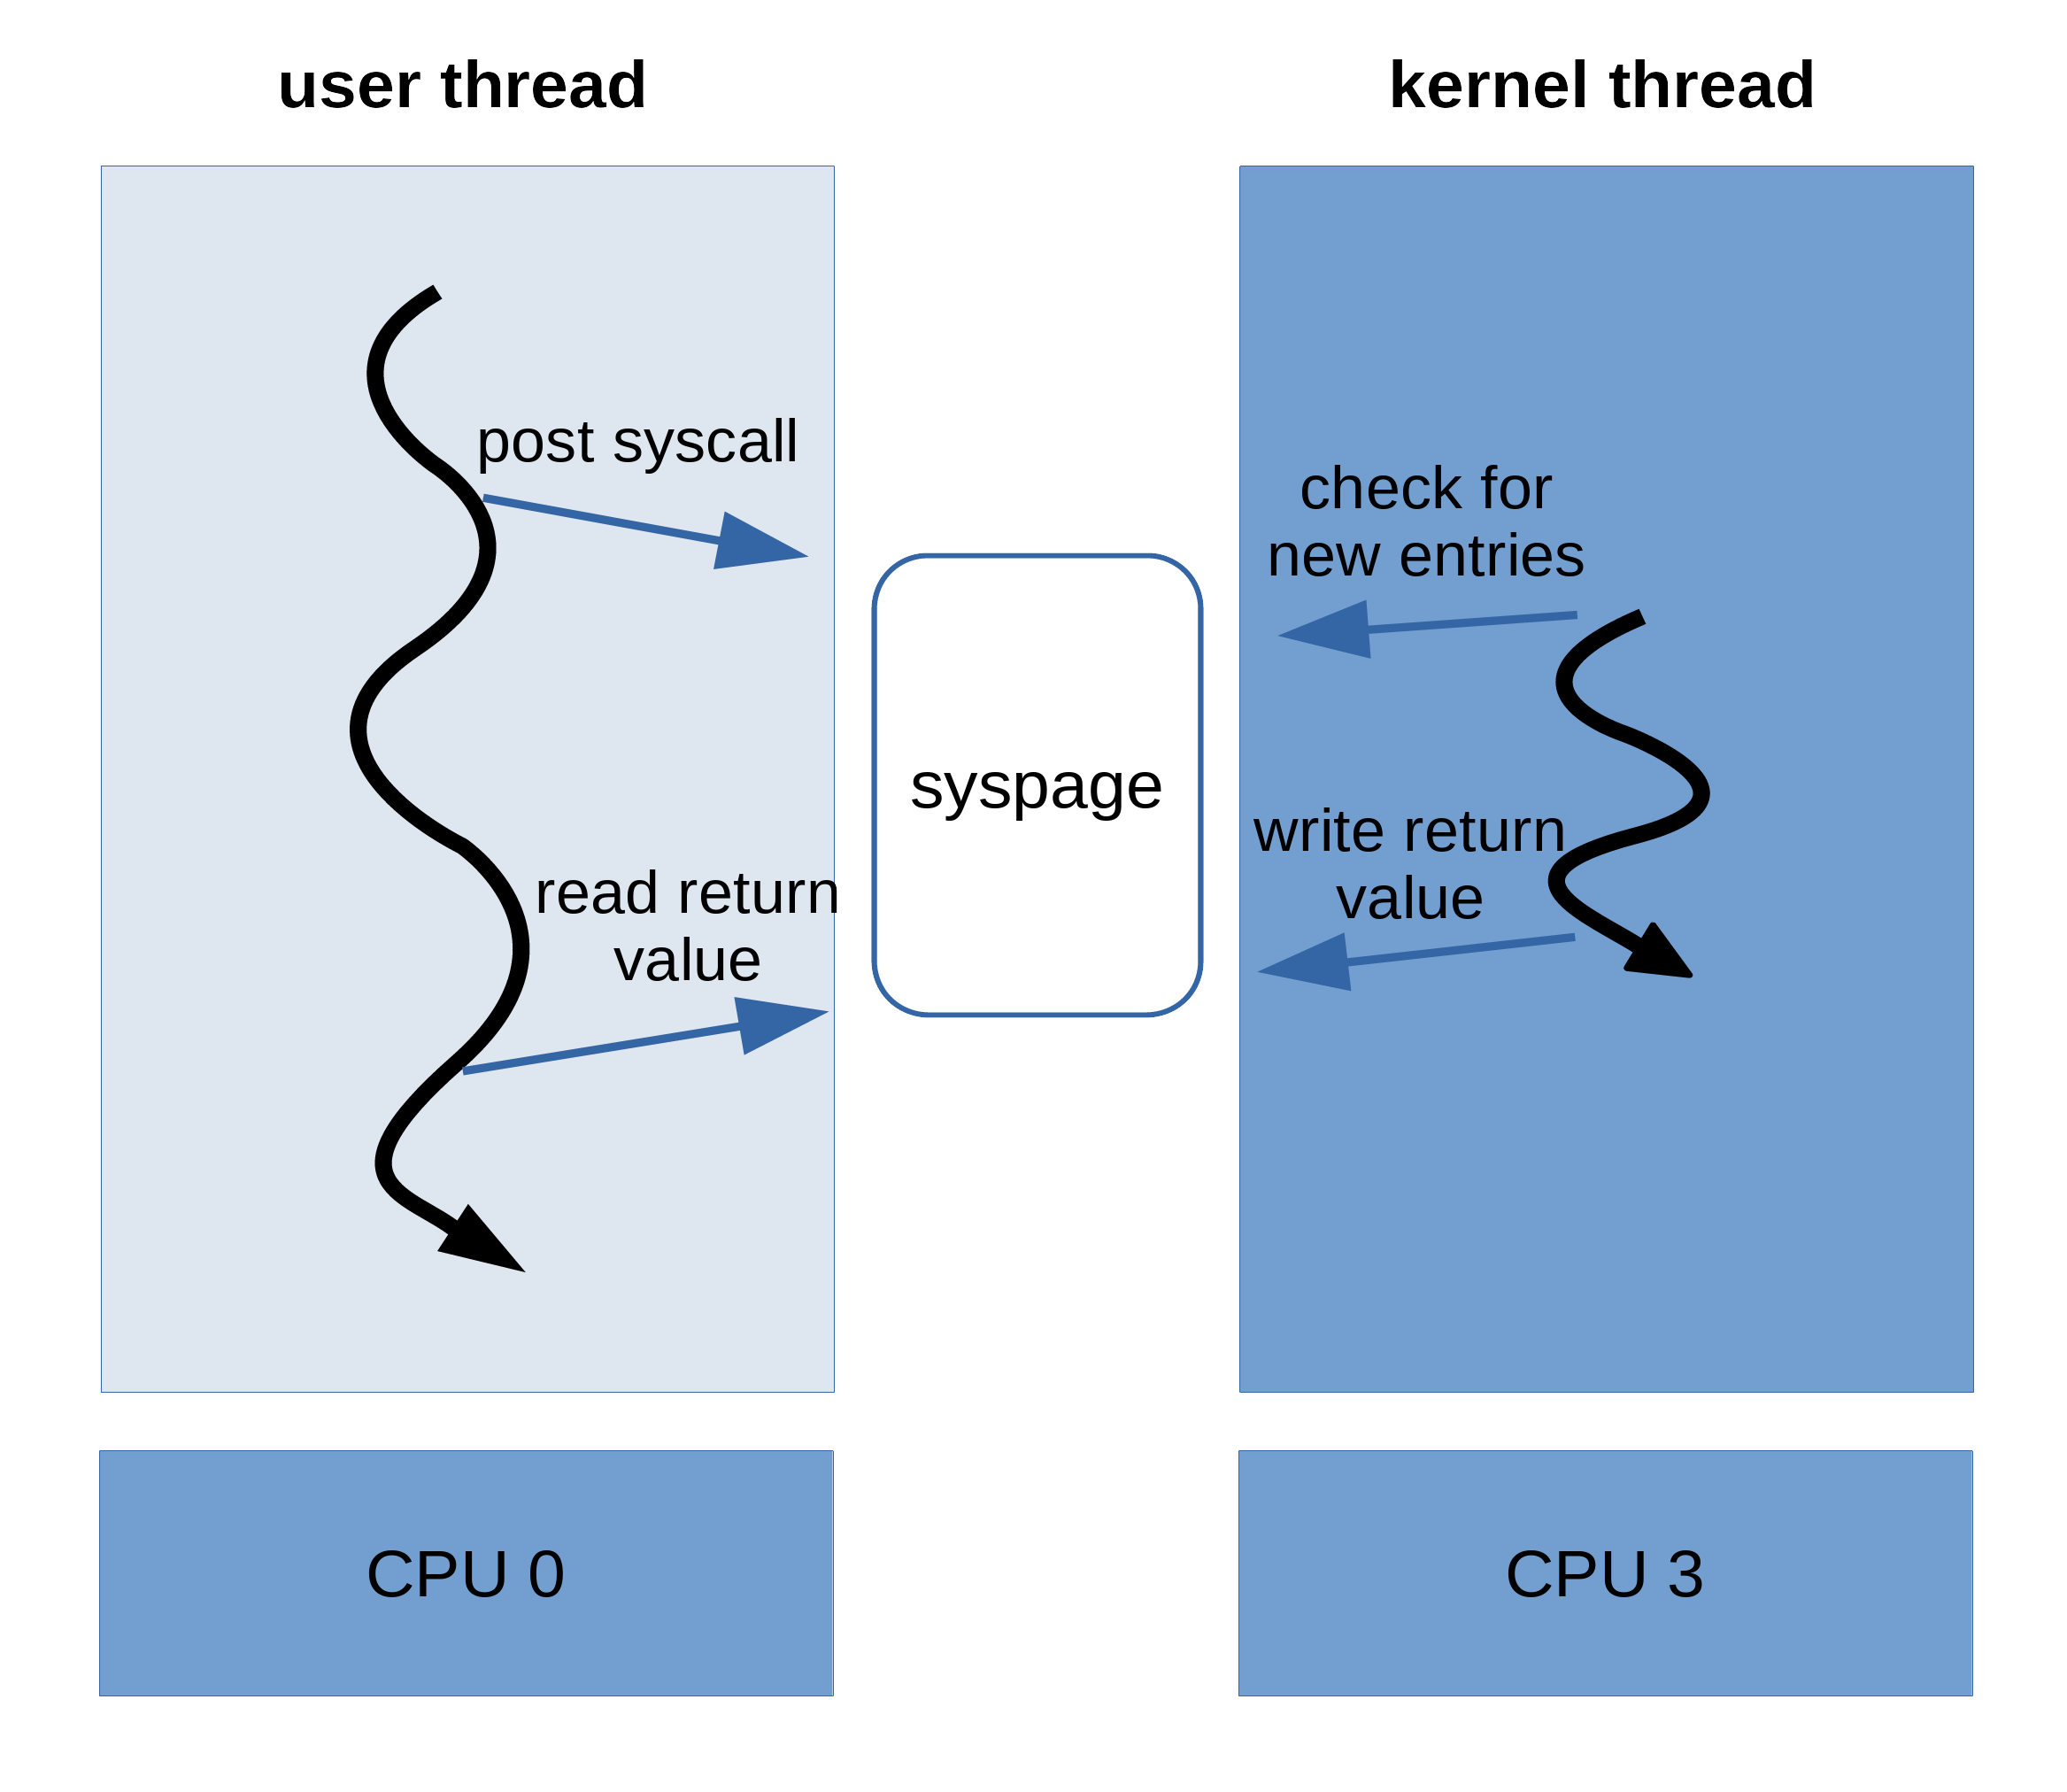
\includegraphics[scale=0.13]{code_parallel}
  \caption{Parallel execution of user-space and kernel-space code for the same
  process. On the left is a decoupled \llinux thread and on the right its
  corresponding \memsc worker executing its system calls in parallel on a
  separate CPU.}
\label{fig:code_parallel}
\end{figure}

\break

Since system calls and exceptions are forwarded separately, it is even possible
that different kernel code for the same process is executed in parallel. For
example, if the decoupled thread posts a few system calls and then generates a
page fault, there can be a situation where the memsc worker and the kernel-side
context run in parallel. In order for this to happen, there would need to be
enough available vCPUs running on separate physical CPUs. In that case, no
user-space progress would be made since exceptions cannot be dealt with
asynchronously.

\section{Using \memsc}

There are two ways of using the new \memsc forwarding mechanism. One is by
directly invoking the \memsc user-space library and the other one is by using
it indirectly via a modified version of the C library. This section presents
\lib and its API through which applications can take full advantage of all
\memsc capabilities.

\subsection{The \memsc User-Space Library}

User applications can benefit from the new forwarding mechanism using
\emph{\lib}, the \memsc user-space library. This library can be linked
dynamically in programs or it can be statically linked during compilation time.
Applications can then call the functions offered by its public interface
directly.

Using \lib requires source code modifications for existing applications.
Therefore this approach is more suitable for new applications or for smaller
existing programs for which porting them would not require significant efforts.

By using \lib directly, an application can take full advantage of all of the
\memsc mechanism's capabilities. In particular, it is the only way for an
application to use system call batching and asynchronous system calls that
allow parallel execution of user and kernel code as described in the previous
section. Hence, using \lib directly is especially suitable for applications
that can be designed in advance (or be ported) to batch system calls and
benefit from their asynchronous execution.

\subsection{Application Interface (memsclib API)}

User programs that are linked against \lib and include the appropriate header
file can make use of the following interfaces.

\break

{\parindent0pt % disables indentation for all the text between { and }

\textbf{int memsc\_register()}

{\addtolength{\leftskip}{5mm}

This function is used by a user process in order to register for \memsc
services. It needs to be called prior to any other \memsc-related function. A
new \sysp is created as a result of that call along with a worker thread for
that process.

On success 0 is returned, otherwise an integer indicating an error.

}

\textbf{memsc\_idx memsc\_add(int sysno, ...)}

{\addtolength{\leftskip}{5mm}

This function is used for posting new system calls in the \sysp. The new entry
is added to the first free slot of the ring buffer.

On success, an identifier that refers to a specific slot in the \sysp is
returned. This identifier needs to be passed to other \lib calls.

}

\textbf{bool memsc\_ready(memsc\_idx idx)}

{\addtolength{\leftskip}{5mm}

This function returns true when the entry referred to by \emph{idx} has been
processed by the kernel and the result is available. A process can busy-wait by
repeatedly calling this function if it cannot proceed otherwise without having
the result of the system call.

}

\textbf{long memsc\_retval(memsc\_idx idx)}

{\addtolength{\leftskip}{5mm}

This function returns the system call's return value stored by the kernel in
the entry referred to by \emph{idx}. This function must be called only after
\emph{memsc\_ready()} for the same entry has returned true. It must be called
only once for a given index as it results in its slot being freed.

}

\textbf{void memsc\_wait\_all()}

{\addtolength{\leftskip}{5mm}

Calling this function blocks execution of the calling thread until all of the
posted system calls have been processed by the kernel.

}

\textbf{void memsc\_wait\_any()}

{\addtolength{\leftskip}{5mm}

Calling this function blocks execution of the calling thread until one or more
of the posted system calls have been processed by the kernel.

}

} % restore indentation

\subsection{Examples}

Using the \lib API presented above, applications can invoke system calls in
both an asynchronous and a synchronous manner.

\begin{figure}[h]
    \begin{lstlisting}[language=C, breaklines=false]
#include "memsclib.h"

	...

	if (memsc_register())
		return -1;

	memsc_idx m_open = memsc_add(__NR_open, "file", 0, "r");

	while (!memsc_ready(m_open));

	int fd = memsc_retval(m_open);

	...
    \end{lstlisting}
    \caption{Example of a synchronous blocking system call invocation using
    \memsc}
    \label{fig:example_sync}
\end{figure}

Figure \ref{fig:example_sync} shows an example of issuing a traditional,
blocking system call using \lib. Before doing anything else, the application
needs to register for \memsc services using the \emph{memsc\_register()} call.
If the call succeeds, the application proceeds with posting an \emph{open}
system call in its \sysp using \emph{memsc\_add()} and then performs busy
waiting in line 10 until the result of the system call invocation is available.
Finally, it consumes the value by copying it back to its stack before
proceeding with its execution.

\begin{figure}[h]
    \begin{lstlisting}[language=C]
	...

	memsc_add(__NR_write, fd1, str, strlen(str));
	memsc_add(__NR_write, fd2, str, strlen(str));
	memsc_add(__NR_write, fd3, str, strlen(str));
	memsc_add(__NR_write, fd4, str, strlen(str));

	memsc_wait_all();

	...
    \end{lstlisting}
    \caption{Example of system call batching using \memsc}
    \label{fig:example_batch}
\end{figure}

Figure \ref{fig:example_batch} shows an example of system call batching using
\lib. This time the application posts 4 \emph{write} system calls to different
file descriptors it already holds. It then blocks using the
\emph{memsc\_wait\_all()} library call. Once this call returns, it means that
all system calls posted until the time of the call have been completed and
their results can be collected.

\section{Using \memsc Transparently}

Since porting existing applications to use \lib can often be prohibitive, using
memsclib directly is not always an option. In this case, another way of using
\memsc services without modifying existing programs is offered. This is
achieved with the help of a slightly modified version of the C library that
enables \memsc usage and has been adjusted for this purpose.

Thanks to the dynamic loading capabilities of Linux, the whole process is
completely transparent to applications. Existing programs simply need to link
against the modified C library and they can then call the library's system call
wrappers as usual. These wrappers, instead of setting up the CPU registers and
raising an exception, they make calls to \lib.

Due to the fact that the C library semantics imply blocking system calls, using
\memsc this way does not allow for asynchronous system calls and system call
batching. However, even in this case, \llinux applications running decoupled on
a separate core should experience improved performance nevertheless since all
system calls are forwarded via the \sysp{s}.
